\documentclass[12pt]{article}
\usepackage{amssymb}
\usepackage{amsmath}
\usepackage{graphicx}
\usepackage{geometry}

\begin{document}
\centerline{MASSACHUSETTS INSTITUTE OF TECHNOLOGY}
\centerline{Physics Department}
\noindent Physics 8.S10 \hfil Spring Semester 2018\break


\centerline{\bf Lab Report: Default Lab on March 9, 2018} % add lab name and date
\centerline{Authors: \underline{Jane Doe}, Jim Smith}     % underline your own name
                                                          % add your lab partner as author

\section{Introduction}

Give a motivation of the work described in the following and what the
theoretical background is. Any of your lab partners should be able to follow but
more importantly any other physicist who would like to use you results or maybe
repeat or even improve on them.

\section{Experimental Setup}

Describe the experimental setup and highlight the salient features that you are
later refering to in the analysis of you data and the discussion of the
uncertainties in particular. A picture of the experimental setup, like the one
in Figure~\ref{fig:myPngExample}, helps a lot with the desciption.

\begin{figure}[htbp!]
  \centering
  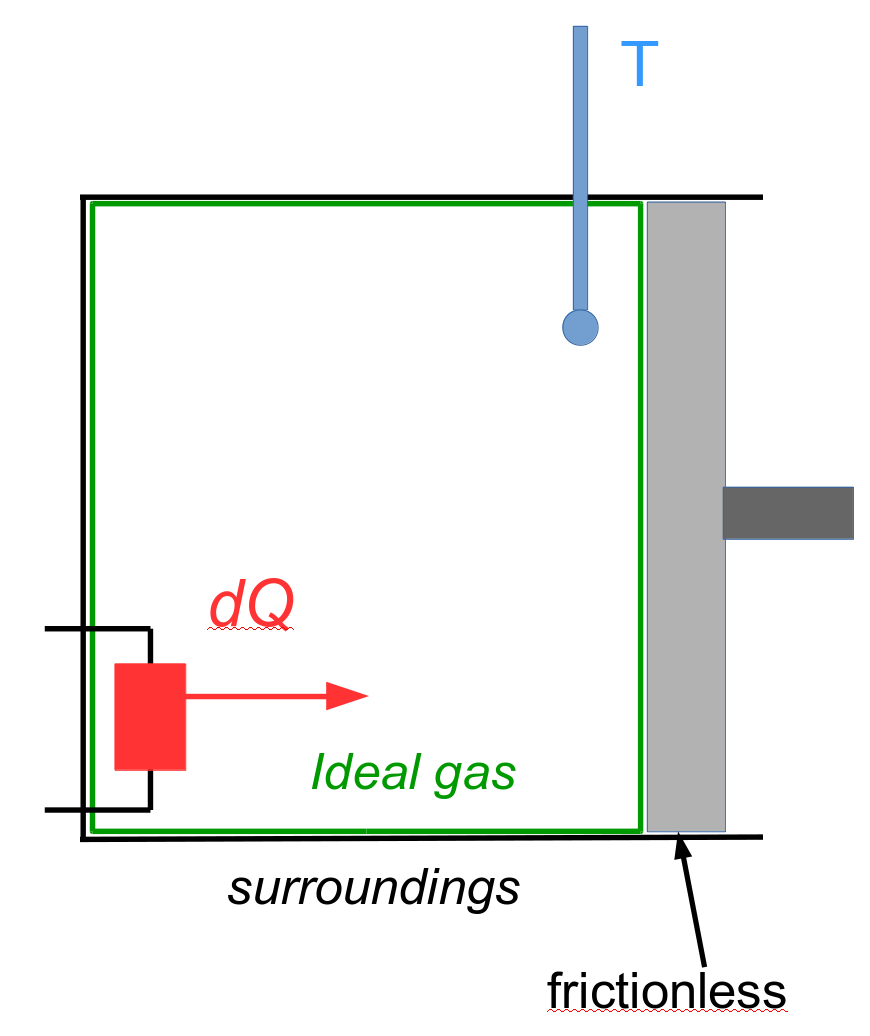
\includegraphics[width=0.4\textwidth]{myPngExample1.png}~~~~~~~~~~~~~
  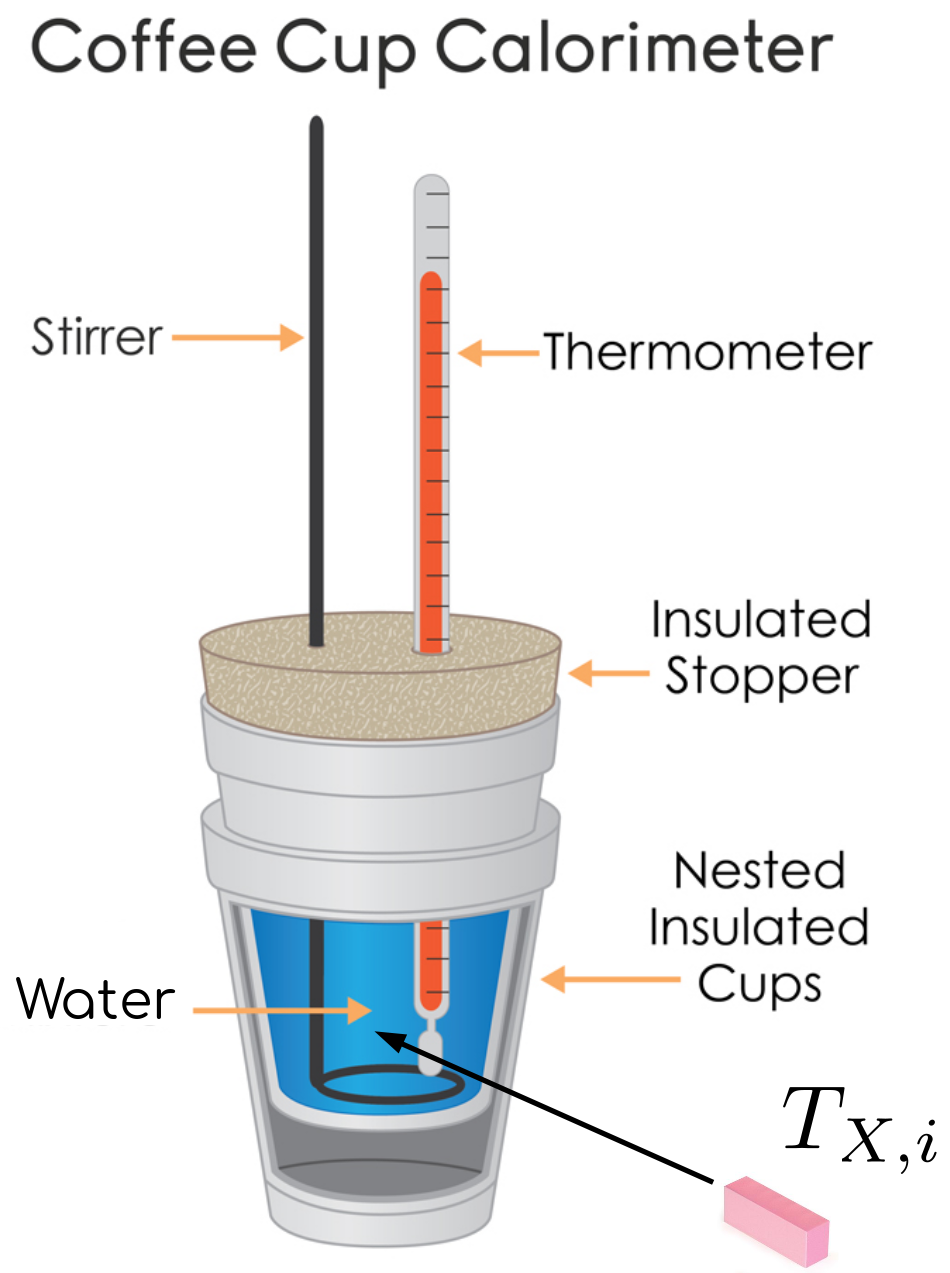
\includegraphics[width=0.4\textwidth]{myPngExample2.png}
  \caption{\label{fig:myPngExample}
    These are two example figures.
  }
\end{figure}

\section{Data Presentation and Analysis}

You should present the data and how you collected them, so that the reader can
follow your analysis. The raw data is ususally shown and then the analysis
perfromed on those data is described.

Uncertainties that you want to include you have to first motivate. Then you
describe the way you want to evalute them and finally you derive the number
following the recipe given.

\section{Conclusion}

The conclusion is a succinct summary of the results, but beyond that it will
discuss their meaning in the bigger context and comment on their scientific
meaning.

\end{document}
